\documentclass[14pt, a4paper]{article}



%%%%%%%%%%%%%%%%%%%%%%%% Шрифты %%%%%%%%%%%%%%%%%%%%%%%%%%%%%%%%%
\usepackage{fontspec}         % пакет для подгрузки шрифтов
\setmainfont{Arial}   % задаёт основной шрифт документа

% Команда, которая нужна для корректного отображения длинных тире и некоторых других символов.
\defaultfontfeatures{Mapping=tex-text}

% why do we need \newfontfamily:
% http://tex.stackexchange.com/questions/91507/
\newfontfamily{\cyrillicfonttt}{Arial}
\newfontfamily{\cyrillicfont}{Arial}
\newfontfamily{\cyrillicfontsf}{Arial}

\usepackage{polyglossia}      % Пакет, который позволяет подгружать русские буквы
\setdefaultlanguage{russian}  % Основной язык документа
\setotherlanguage{english}    % Второстепенный язык документа


%%%%%%%%%% Работа с картинками %%%%%%%%%
\usepackage{graphicx}                  % Для вставки рисунков



%%%%%%%%%% Гиперссылки %%%%%%%%%%
\usepackage{xcolor}              % разные цвета


\usepackage{hyperref}
\hypersetup{
    colorlinks=true,       	% true - цветные ссылки, false - ссылки в рамках
    urlcolor=blue,          % цвет ссылки на url
}


\usepackage{setspace}
\usepackage[paper=a4paper,top=10mm, bottom=10mm,left=35mm,right=35mm,includefoot,includehead]{geometry}
\setstretch{1}  % Межстрочный интервал
\usepackage{extsizes} %чтобы подгрузить 14 шрифт
\setlength{\parskip}{4mm}   % Расстояние между абзацами
\setlength{\parindent}{0em} % Красная строка

\usepackage{fancyhdr} % Колонтитулы
\pagestyle{fancy}

%%%%%%Секции и колонтитулы%%%%%%%%
\usepackage{titlesec} 
\titleformat{\section}{\Large\bfseries}{Приложение \Asbuk{section}:}{10pt}{}
\renewcommand{\headrulewidth}{0.2pt}
\renewcommand{\sectionmark}[1]{\markright{%
\MakeUppercase{Приложение \Asbuk{section} \hspace{5pt} #1}}}
	\rhead{\thepage}
	\lhead{\rightmark}
	\cfoot{Школа Чародейства и Волшебства <<Хогвартс>>} % номер страницы

\newcommand*{\MyPoint}{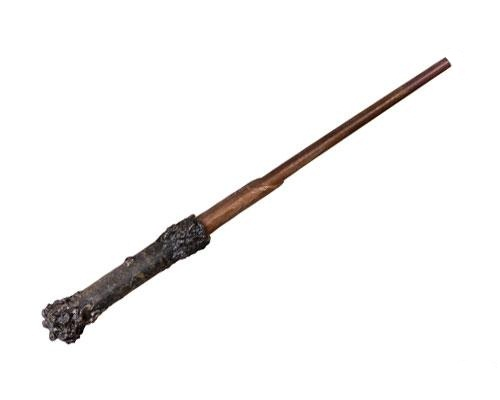
\includegraphics[scale=0.05]{volsh.jpg}}
\renewcommand{\labelitemi}{\MyPoint}


\begin{document}
\newgeometry{top=10mm, bottom=10mm,left=35mm,right=35mm}
\thispagestyle{empty}

\begin{figure}[t]
\begin{center}

\includegraphics[height=6cm,width=8cm,keepaspectratio]{gerb.png}
\end{center}
\end{figure}

\vspace{1cm}

{ \fontsize{12}{1}\selectfont Дорогой мистер Куц!}

\vspace{2.5cm}

Мы рады проинформировать Вас, что Вам предоставлено место в Школе чародейства и волшебства «Хогвартс». Пожалуйста, ознакомьтесь с приложенным к данному письму списком необходимых книг и предметов. \\
Занятия начинаются 1 сентября. Ждем вашу сову не позднее 31 июля. \par
Искренне Ваша, \\
{\fontspec{NinaCTT}{Minerva McGonagall}} \\
заместитель директора

\vfill
\begin{center}
ШКОЛА ЧАРОДЕЙСТВА И ВОЛШЕБСТВА «ХОГВАРТС»\\
Директор: Альбус Дамблдор\\
(Кавалер ордена Мерлина I степени, Великий волшебник, Верховный чародей, Президент Международной конфедерации магов)\\
\href{http://hogwarts.ru/}{Здесь} можно найти сайт.
\end{center}
\clearpage
\restoregeometry

\section{Список необходимых книг и предметов}

\begin{itemize}
\item Волшебная палочка - 1шт.
\item Оловянный котёл, стандартный размер №2 - 1шт.
\item Комплект стеклянных или хрустальных флаконов - 1шт.
\item Телескоп - 1шт.
\item Медный весы - 1шт.
\item Чёрные простые рабочие мантии - 3шт.
\item Чёрная простая остроконечная шляпа на каждый день - 1шт.
\item Сова, кошка или жаба - при желании
\item «Курсическая книга заговоров и заклинаний» (первый курс) Миранда Гуссокл
\item «История магии». Батильда Бэгшот
\item «Теория магии». Адальберт Уоффлинг
\item «Пособие по трансфигурации для начинающих». Эмерик Свитч
\item «Тысяча магических растений и грибов». Филли-да Спора
\item «Магические отвары и зелья». Жиг Мышъякофф
\item «Фантастические звери: места обитания». Ньют Саламандер(Скамандер)
\item «Темные силы: пособие по самозащите».Квентин Тримбл
\end{itemize}

\newpage
\section{Список изучаемых предметов}

\begin{itemize}
\item Астрономия
\item Заклинания
\item Зельеварение
\item История магии
\item Травология
\item Трансфигурация
\item Полёты на мётлах
\item Защита от Тёмных искусств
\end{itemize}


\end{document}